96. а) $f(x)=\begin{cases} \cfrac{3x-1}{x+1},\ x
eq-1\\3+2,\ x=-1 \end{cases}=\begin{cases} 3-\cfrac{4}{x+1},\ x
eq-1\\5,\ x=-1 \end{cases}.$
$$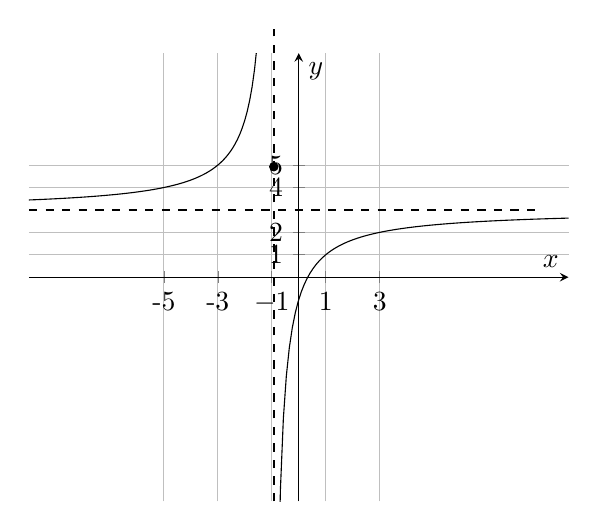
\begin{tikzpicture}[scale=1]
\tikzset{line03/.style={dashed,line width =0.9pt}}
\begin{axis}[
    axis lines = middle,
    grid=major,
    legend pos={south west},
    xlabel = {$x$},
    %xlabel style={below right},
    ylabel = {$y$},
    ymin=-10,
    ymax=10,
    xmin=-10,
    xmax=10,
    xtick={-5, -3, -1, 1, 3},
    xticklabels={-5, -3, $\text{                     -1}$, 1, 3},
    ytick={4, 5, 1, 2},
    yticklabels={$\text{4          }$,$\text{5           }$, $\text{1          }$, $\text{2            }$},        ]

	\addplot[domain=-0.9:10, samples=100, color=black] {3-4/(x+1)};
	\addplot[domain=-10:-1.1, samples=100, color=black] {3-4/(x+1)};

\end{axis}
\filldraw [black] (3.11,4.25) circle (1.5pt);
\draw[line03] (3.11,0) -- (3.11,6);
\draw[line03] (0,3.7) -- (6.5,3.7);
%\draw (3,5.7) node {\scriptsize $y$};
%\draw (7,2.5) node {\scriptsize $x$};
\end{tikzpicture}$$
б) Горизонтальная прямая $y=a-1$ не пересекается с графиком данной функции только в том случае, если является его асимптотой, то есть $a-1=3,\ a=4.$\\
в) Прямая $y=ax+1$ имеет с графиком три общие точки, только если она пересекает гиперболу 2 раза (тогда $a<0$) и проходит через изолированную точку $(-1;a+2).$ Тогда $-a+1=a+2,\ 2a=-1,\ a=-\cfrac{1}{2}.$\\
